\ifx\allfiles\undefined

	% 如果有这一部分另外的package,在这里加上
	% 没有的话不需要
	
	\begin{document}
\else
\fi
    \chapter{非线性规划}
    \section{非线性规划问题与数学模型}
    \subsection{非线性规划问题的定义}
    
\begin{dfnbox}{非线性规划}{amznotes}
    如果目标函数或约束条件方程中存在任何非线性因子,则问题\textbf{非线性规划}。
\end{dfnbox}
非线性规划具有以下几个特点:
\begin{itemize}
    \item 目标函数或约束条件方程中存在任何\textcolor{red}{非线性因子},或全部为\textcolor{red}{非线性函数}:
    \item \textcolor{red}{没有统一的、通用的解法}(这不同于线性规划,它有单纯形法作为通用解法),目前各种解法都有自己的适用范围;
    \item 非常难以采用解析解法,更多采用\textcolor{red}{数值解法};
    \item 非线性规划的最优解不像线性规划那样在边界点达到,而是\textcolor{red}{有可能在可行域中任一点}达到;
    \item 非线性规划存在\textcolor{red}{局部极值点}和\textcolor{red}{全局极值点}之分,这一点也与线性规划不同。
\end{itemize}
\begin{dfnbox}{局部极值点}{amznotes}
    设 $x^* \in K$,如果存在某个 $\epsilon > 0$,使得有与 $x$ 距离小于 $\epsilon$ 的 $x \in K$(即 $x \in K \cap \|x - x^*\| < \epsilon$),均满足不等式 $f(x) \geq f(x^*)$,则称 $x^*$ 为 $f(x)$ 在 $K$ 上的局部极小点,$f(x^*)$ 为局部极小值。\\
    若 $x \neq x^*$ 且 $f(x) > f(x^*)$,则 $x^*$ 为严格局部极小点,$f(x^*)$ 为严格局部极小值。
\end{dfnbox}
\begin{dfnbox}{全局极值点}{amznotes}
    设 $x^* \in K$,如果对于任意 $x \in K$,都有 $f(x) \geq f(x^*)$,则称 $x^*$ 为 $f(x)$ 在 $K$ 上的全局极小点,$f(x^*)$ 为全局极小值。\\
    若 $x \neq x^*$ 且 $f(x) > f(x^*)$,则 $x^*$ 为严格全局极小点,$f(x^*)$ 为严格全局极小值。
\end{dfnbox}
两点说明:
\begin{itemize}
    \item 局部极值点和全局极值点在定义上的主要区别是点的比较范围是x*附近的一个小邻域,还是整个K域。
    \item 局部极小点可能同时是全局极小点,全局极小点同时一定是局部极小点。
\end{itemize}
\begin{figure}[H]
    \centering
    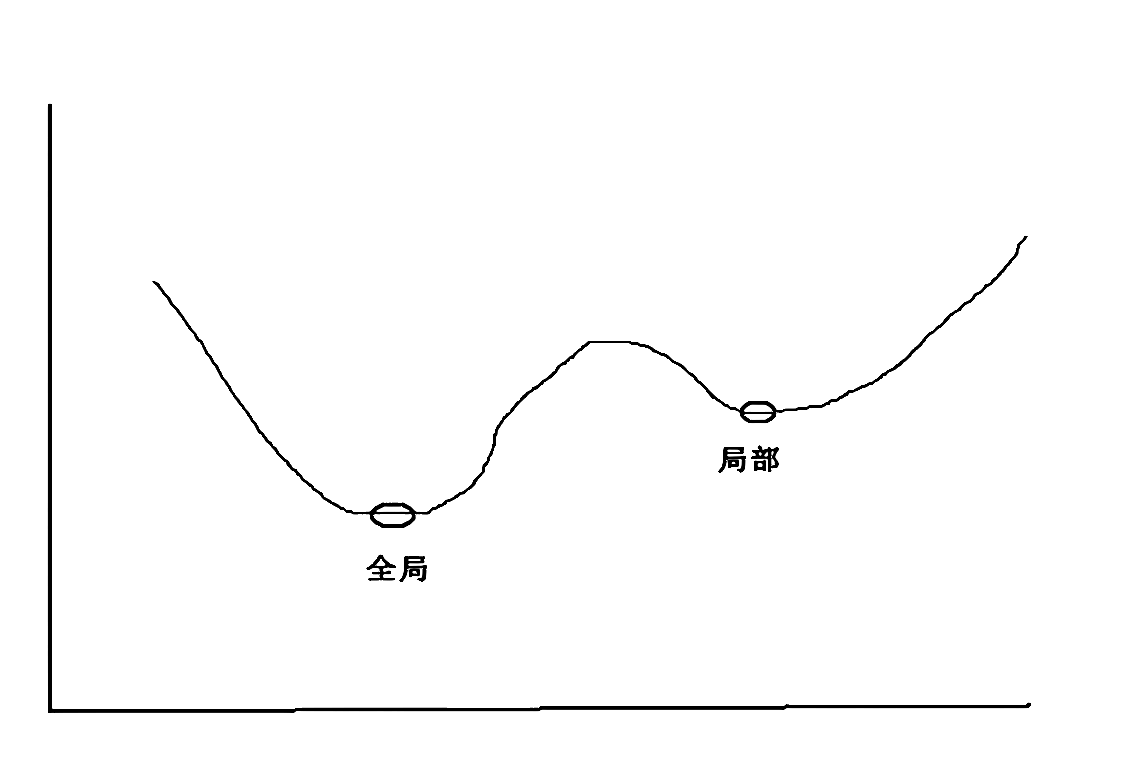
\includegraphics[width=0.5\textwidth]{./image/19.png}
    \caption{非线性规划也有局部极值和全局极值的区分}
    \label{fig:Chapter4_Temporary_Pavilion_1}
\end{figure}
\begin{figure}[H]
    \centering
    \begin{subfigure}{0.42\textwidth}
        \centering
        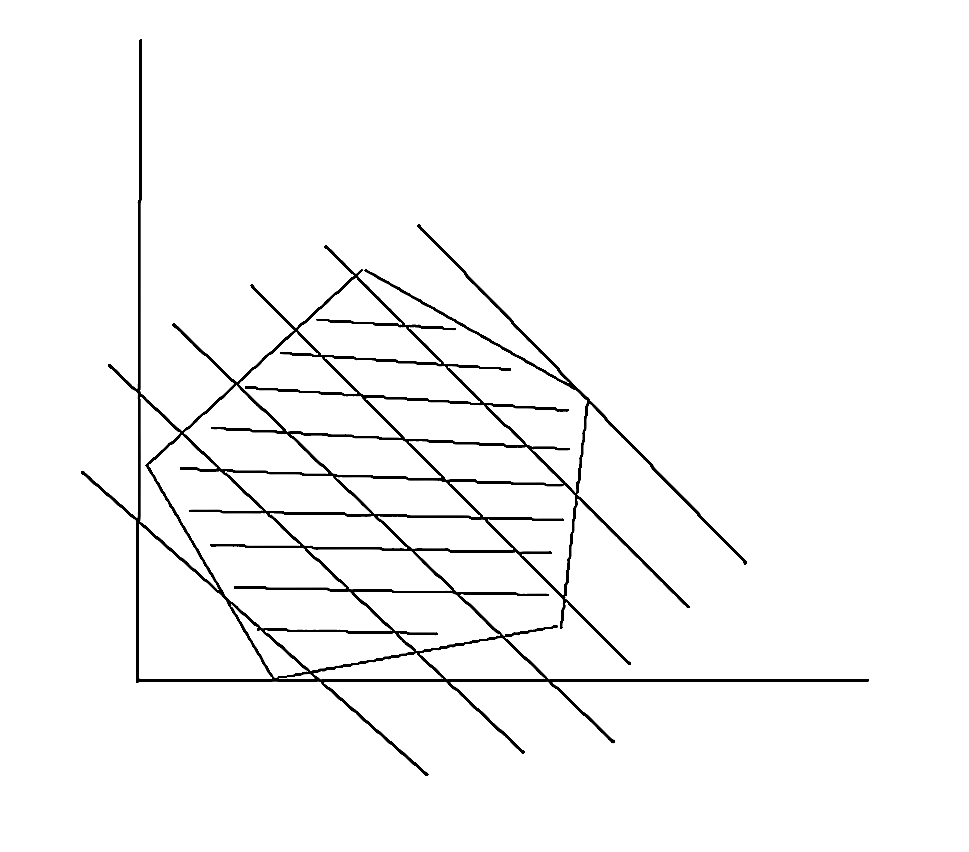
\includegraphics[width=\linewidth]{image/17.png}
        \caption{线性规划中,当目标函数取定值时,其等值几何图形为直线或平面。}
    \end{subfigure}
    \hfill
    \begin{subfigure}{0.4\textwidth}
        \centering
        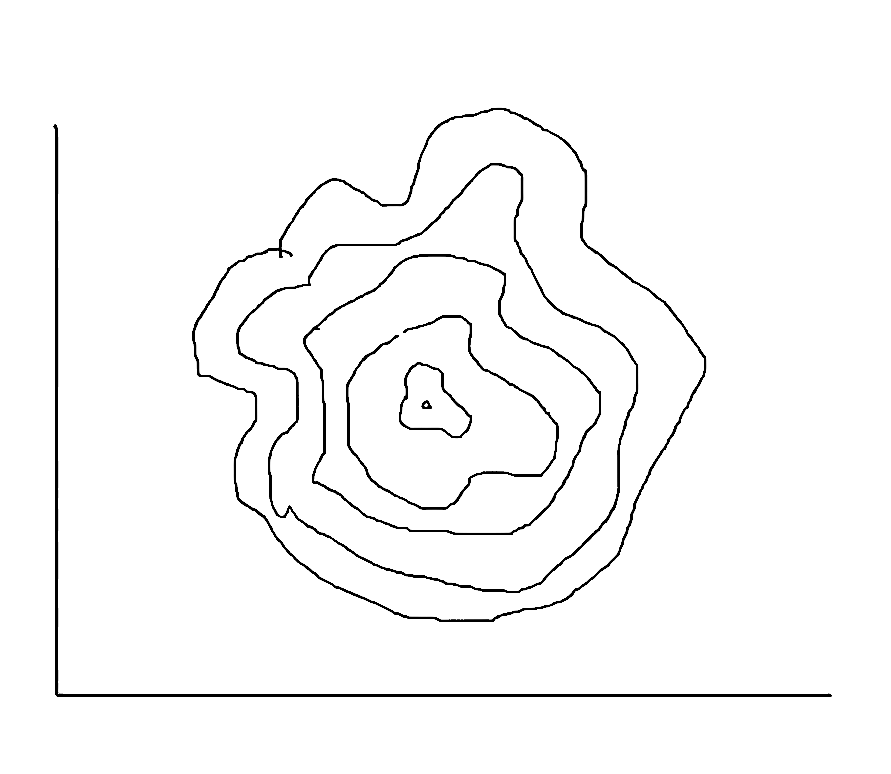
\includegraphics[width=\linewidth]{image/18.png}
        \caption{非线性规划中,等值线为规则或不规则的曲线、曲面,类似于地图上的等高线}
    \end{subfigure}
    \caption{线性规划与非线性规划的对比}
\end{figure}

\begin{exbox}{资源分配问题}
1\textbf{例:}有 A 和 B 两种资源,数量分别为 a 和 b,用于生产 n 种产品。如果 A 种资源以数量 \(x_k\),B 种资源以数量 \(y_k\),用于生产第 k 种产品,其收益为 \(g_k(x_k, y_k)\),问如何分配这两种资源用于 n 种产品的生产使总收益最大?
\\
\textbf{解:}

由题意,以 \(x_k\) 和 \(y_k\)(\(k = 1, 2, \dots, n\))为决策变量,以生产 n 种产品的总收益为目标函数,资源的总量为约束条件,则问题的优化模型为:

\[
\max z = g_1(x_1, y_1) + g_2(x_2, y_2) + \dots + g_n(x_n, y_n)
\]

约束条件:

\[
\begin{cases}
x_1 + x_2 + \dots + x_n = a, \\
y_1 + y_2 + \dots + y_n = b, \\
x_k \geq 0, \quad y_k \geq 0 \quad (k = 1, 2, \dots, n).
\end{cases}
\]
\end{exbox}

\begin{exbox}{最小圆盘问题}
    1\textbf{例:}设平面上有 $m$ 个点,找覆盖这 $m$ 个点的最小圆盘。

    \textbf{解:} 设 $m$ 个点为 $p_i, \, i = 1, 2, \dots, m$,则平面上任一点 $x$ 到这 $m$ 个点的距离最大者满足
    
    \[
    f(x) = \max_{1 \leq i \leq m} \| x - p_i \|
    \]
    
    则以 $x$ 为圆心,$f(x)$ 为半径的圆盘必覆盖这 $m$ 个点,于是问题转化为求解最小半径的圆盘问题:
    
    \[
    \min_x \max_{1 \leq i \leq m} \| x - p_i \|
    \]
    
    这是一个无约束的非线性规划问题。
\end{exbox}
\textcolor{red}{若没有约束条件,称为无约束极值问题。否则称为约束极值问题。}
\subsection{非线性规划问题的数学模型}
\begin{thmbox}{一般形式}{cool}
    \begin{align*}
        \text{max} \quad & z = g_1(x_1, y_1) + g_2(x_2, y_2) + \cdots + g_n(x_n, y_n) \\
        \text{subject to} \quad & \sum_{k=1}^{n} x_k = a, \\
        & \sum_{k=1}^{n} y_k = b, \\
        & x_k \geq 0, \ y_k \geq 0 \quad (k = 1, 2, \dots, n).
        \end{align*}
        
        \begin{align*}
        \text{min} \quad & \max_{1 \leq l \leq m} \left\{ \| x - p_l \| \right\}
    \end{align*}
\end{thmbox}
\begin{thmbox}{标准模型I}{cool}
    \begin{align*}
        \min \quad & f(x) \\
        \text{subject to} \quad & h_i(x) = 0, \quad i = 1, 2, \dots, m \quad \text{(m 个等式约束)} \\
        & g_j(x) \geq 0, \quad j = 1, 2, \dots, l \quad \text{(l 个不等式约束)} \\
        & x \in \mathbb{R}^n
        \end{align*}
        
        \bigskip
        \text{若有另一种形式,可以转化为上述形式,例如:}
        \begin{align*}
        \max \quad  f(x) \quad &\Rightarrow \quad \min (-f(x)) \\
        g_j(x) \leq 0  \quad &\Rightarrow \quad -g_j(x) \geq 0
        \end{align*}
\end{thmbox}
\begin{thmbox}{标准模型II}{cool}
    \begin{align*}
        \min \quad & f(x) \\
        \text{subject to} \quad & g_i(x) \geq 0, \quad i = 1, 2, \dots, n \quad \text{(n 个不等式约束)} \\
        & x \in \mathbb{R}^n
    \end{align*}
\end{thmbox}


\begin{notebox}{\textbf{模型 I 与模型 II 的转换:}}
\\
主要是把等式约束化为不等式约束:
\begin{align*}
    h_i(x) = 0 \quad \Rightarrow \quad \begin{cases}
        h_i(x) \geq 0 \\
        h_i(x) \leq 0 \quad \Rightarrow \quad -h_i(x) \geq 0
    \end{cases}
    \Rightarrow
    g_i(x)\geq 0 
\end{align*}
\end{notebox}
\begin{notebox}{\textbf{求解方法}}
    \\求解非线性规划问题常有两种方法:
    \begin{enumerate}
        \item \textbf{解析法}:必要条件+充分条件;
        \item \textbf{数值法}:迭代。
    \end{enumerate}
\end{notebox}


\subsection{求解非线性规划问题的解析法}
为了使用解析方法解决非线性规划问题,我们首先引出几个定义\footnote{读者在微积分或数学分析课程中中学过以上概念。如果感到有些遗忘,可以理解为“梯度”就相当于一元函数的一阶导数,“Hesse 矩阵”就相当于一元函数的二阶导数。我们在判断一元函数的极值点的时候,就是通过求一阶导为0,二阶导大于或小于0来判断是极小值或极大值的。对于多元函数也是类似的道理。}:
\begin{dfnbox}{函数的梯度}{amznotes}
    设 $x \in K \subset \mathbb{R}^n$,$f(x)$ 在 $K$ 上有一阶连续偏导数,则
    \[
    \nabla f(x) \equiv \left[ \frac{\partial f(x)}{\partial x_1}, \frac{\partial f(x)}{\partial x_2}, \ldots, \frac{\partial f(x)}{\partial x_n} \right]^T
    \]
    称函数 $f(x)$ 在 $x$ 处的\textbf{梯度}。
\end{dfnbox}
\textbf{梯度的几何意义}:
    $\nabla f(x)$ 是 $f(x)$ 在 $x$ 处增加最快或减少最快的速度,也是 $f(x)$ 的图形在 $x$ 处的陡峭程度。
\begin{dfnbox}{平稳点}{amznotes}
    若$\nabla f(x)=0$,则称$x$是$f(x)$的\textbf{平稳点}。
\end{dfnbox}

\begin{dfnbox}{海森Hesse矩阵}{amznotes}
    设 $f(x)$ 在 $K$ 上有二阶连续偏导数,则
    \[
    H(x) \equiv \begin{bmatrix}
        \frac{\partial^2 f(x)}{\partial x_1^2} & \frac{\partial^2 f(x)}{\partial x_1 \partial x_2} & \cdots & \frac{\partial^2 f(x)}{\partial x_1 \partial x_n} \\
        \frac{\partial^2 f(x)}{\partial x_2 \partial x_1} & \frac{\partial^2 f(x)}{\partial x_2^2} & \cdots & \frac{\partial^2 f(x)}{\partial x_2 \partial x_n} \\
        \vdots & \vdots & \ddots & \vdots \\
        \frac{\partial^2 f(x)}{\partial x_n \partial x_1} & \frac{\partial^2 f(x)}{\partial x_n \partial x_2} & \cdots & \frac{\partial^2 f(x)}{\partial x_n^2}
    \end{bmatrix}
    \]
    称函数 $f(x)$ 在 $x$ 处的 \textbf{Hesse 矩阵}。
\end{dfnbox}
\begin{dfnbox}{矩阵的正定性,负定性,不定性}{amznotes}
    对于对称矩阵 $A$,若对任意非零向量 $X \neq 0$,二次型为正,即 $X^T A X > 0$,则称该二次型为正定二次型,$A$ 为正定矩阵\footnote{在线性代数中,我们学习过判断正定矩阵的方法有特征值判定法(所有特征值大于0)、主子式判定法(如果所有阶的顺序主子式,即从左上角开始的子矩阵的行列式都大于0);此外,如果两个矩阵都是正定的,那他们的和也是正定的;一个正定矩阵的逆矩阵也是正定的。}。\\
    若 $X^T A X \geq 0 \Rightarrow$ 半正定\\
    若 $X^T A X < 0 \Rightarrow$ 负定\\
    若 $X^T A X \leq 0 \Rightarrow$ 半负定\\
    若既非正定,又非负定,则为不定。
\end{dfnbox}
\begin{thmbox}{定理一:极值点必要条件}{cool}
    若$f(x)$在其存在一阶连续偏导数的区域内达到局部极值点,则该极值点必为平稳点。
\end{thmbox}
此处要注意:
\begin{itemize}
    \item 该定理是必要条件,反之不一定成立,即\textcolor{red}{平稳点不一定是极值点},例如鞍点。
    \item $f(x)$在其不满足一阶连续偏导数的区域内的极值点,不一定满足定理一。
\end{itemize}
\begin{figure}[H]
    \centering
    \begin{subfigure}{0.42\textwidth}
        \centering
        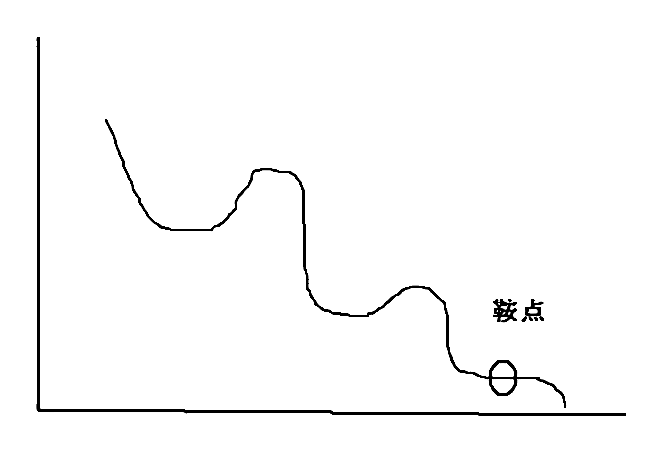
\includegraphics[width=\linewidth]{image/20.png}
        \caption{鞍点是平稳点但不是极值点}
    \end{subfigure}
    \hfill
    \begin{subfigure}{0.4\textwidth}
        \centering
        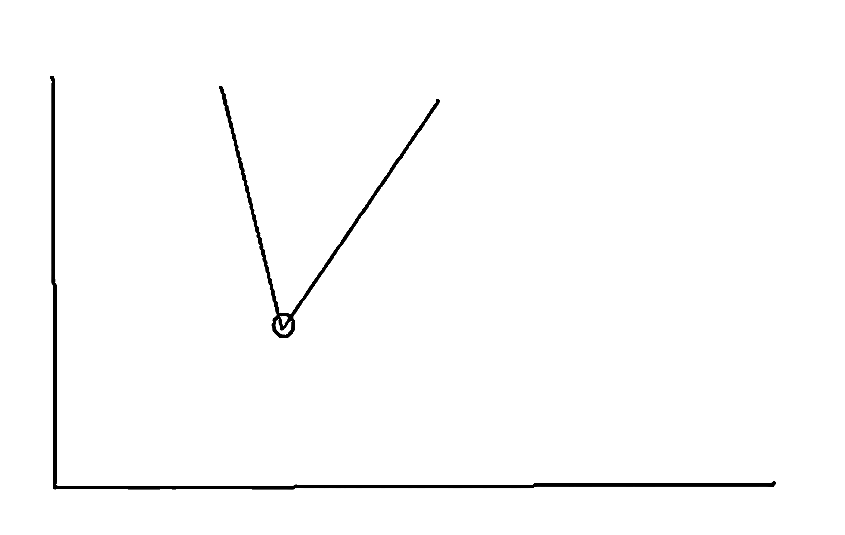
\includegraphics[width=\linewidth]{image/21.png}
        \caption{一阶偏导数不连续的极值点不一定是平稳点}
    \end{subfigure}
    \caption{定理一是必要条件的理解}
\end{figure}
为了能够正确判断极值点,我们使用定理二:
\begin{thmbox}{定理二:局部极值点判断的充要条件}{cool}
    若 $f(x)$ 在 $K$ 上具有二阶连续偏导数,并且满足:
    \begin{enumerate}
        \item $x^* \in K$ 是平稳点,即 $\nabla f(x^*) = 0$
        \item $H(x^*)$ 是正定矩阵(Hesse 矩阵)
    \end{enumerate}
    则 $x^* \in K$ 是 $f(x)$ 的严格局部极小点。
\end{thmbox}
\subsection{求解非线性规划问题的数值法}

\begin{dfnbox}{下降迭代算法}{amznotes}
    若由某算法产生的解序列 $\{ X^{(k)} \}$ 使目标函数值 $f(X^{(k)})$ 逐步减小,则称这组算法为\textbf{下降迭代算法}。
\end{dfnbox}

\begin{notebox}{\textbf{下降迭代算法}}{}
    \begin{itemize}
        \item \textbf{迭代法的基本思路:}
        \\
        初始估计 $X^{(0)}$ \quad $\xrightarrow{\text{按某种算法}}$ \quad 比 $X^{(0)}$ 更好的 $X^{(1)}$ \quad $\xrightarrow{\text{按算法}}$ \quad $X^{(2)} \cdots X^{(n)}$
        $\xrightarrow{\text{得到解序列}} \quad \{ X^{(0)}, X^{(1)}, \cdots, X^{(n)} \cdots \}$
    
        \bigskip
        若解序列收敛于 $X^*$,即,
        \[
        \lim_{k \to \infty} \| X^{(k)} - X^* \| = 0
        \]
        则称 $\{ X^{(0)}, X^{(1)}, \cdots, X^{(n)} \cdots \}$ 收敛于 $X^*$。
        \\
    \end{itemize}
\end{notebox}
几个关键问题是:
\begin{enumerate}
    \item 迭代算法的初始点 $X^{(0)}$ 的选择?
    \item 算法的设计,以当前点依据何种原则构建下一个点?
    \item 迭代算法的终止条件?
\end{enumerate}
\subsubsection{迭代法的基本步骤}
\begin{itemize}
\item \textbf{一、初值的确定}\\初值的确定没有特别的办法,很多情况下依靠经验,或求解者对问题的了解程度来确定的。初值应尽可能与可能的最优解靠得近一些。
\item \textbf{二、算法的设计}
\begin{enumerate}
    \item 选定某一初始点 $X^{(0)}$,并令 $k=0$。

    \item 确定能使 $f(X)$ 下降的搜索方向 $P^{(k)}$。

    \item 从 $X^{(k)}$ 出发行,沿方向 $P^{(k)}$ 确定迭代步长 $\lambda_k$。

    \item 确定,产生下一个迭代点 $X^{(k+1)}$,
    \[
    X^{(k+1)} = X^{(k)} + \lambda_k P^{(k)}.
    \]
    \item 检查新点$X^{k+1}$是否为极小点,或近似极小点,或满足规定的停止条件。
    \begin{itemize}
        \item 若是,则停止迭代;
        \item 否则,令 $k=k+1$,转(2)继续进行迭代。
    \end{itemize}
\end{enumerate}
\textcolor{red}{关键在于如何选取搜索方向 $P^{(k)}$ 和步长 $\lambda_k$}\footnote{各种迭代方法的差异主要就体现在这两者的选定上。}。
\\方向的确定相对困难,但很重要,避免南辕北辙。
\\步长的确定可见\hyperref[确定迭代步长的一维搜索方法]{确定迭代步长的一维搜索方法}和\hyperref[确定迭代步长的黄金分割法]{确定迭代步长的黄金分割法}。
\item \textbf{三、算法的结束条件}
\begin{itemize}
    \item 若算法优秀且收敛的极限值确为最优解,则能通过选代找到最优解。
    \item 若迭代步数有限,只能找到近似解,当满足所要求精度时,即停止迭代。
\end{itemize}
常用以下几个方法:
\begin{enumerate}
    \item \textbf{两次迭代值的绝对误差}
    \[
    \| X^{(k+1)} - X^{(k)} \| < \varepsilon_1
    \]
    \[
    | f(X^{(k+1)}) - f(X^{(k)}) | < \varepsilon_2
    \]

    \item \textbf{两次迭代值的相对误差}
    \[
    \frac{\| X^{(k+1)} - X^{(k)} \|}{\| X^{(k)} \|} < \varepsilon_1
    \]
    \[
    \frac{| f(X^{(k+1)}) - f(X^{(k)}) |}{| f(X^{(k)}) |} < \varepsilon_2
    \]

    \item \textbf{梯度条件}
    \[
    \| \nabla f(X^{(k)}) \| < \varepsilon
    \]
\end{enumerate}
\end{itemize}

\subsubsection{确定迭代步长的一维搜索方法}
\label{确定迭代步长的一维搜索方法}
\begin{notebox}{\textbf{一维、确定步长的三种方法}}
    \begin{enumerate}
        \item \textbf{恒定步长:} 步长每次不变,计算简单,但效果较差。

        \item \textbf{变步长:} 每次人工调整步长,效果较好,但实施麻烦,且需具备较多的经验。

        \item \textbf{最速下降步长:} 使沿搜索方向使目标函数值下降最多、最快,即沿射线 $X = X^{(k)} + \lambda P^{(k)}$ 求使目标函数 $f(X)$ 的极小,
        \[
        \lambda_k : \min f(X^{(k)} + \lambda P^{(k)}),
        \]
        由于这种方法是以$\lambda$为变量的元函数 $f(X^{(k)} + \lambda P^{(k)})$ 的极小点 $\lambda_k$,故称为一维搜索,这种确定的步长为\textbf{最佳步长}。
    \end{enumerate}
\end{notebox}
以下面这个草图为例,从零点出发,方向确定为横轴正方向了,如果在横轴上走出红色的步长,纵轴下降红色的部分;但是如果在横轴走出蓝色的步长,纵轴下降的部分就会更大。这就是先确定方向,沿着搜索方向使目标函数值下降最多。
\begin{figure}[H]
    \centering
    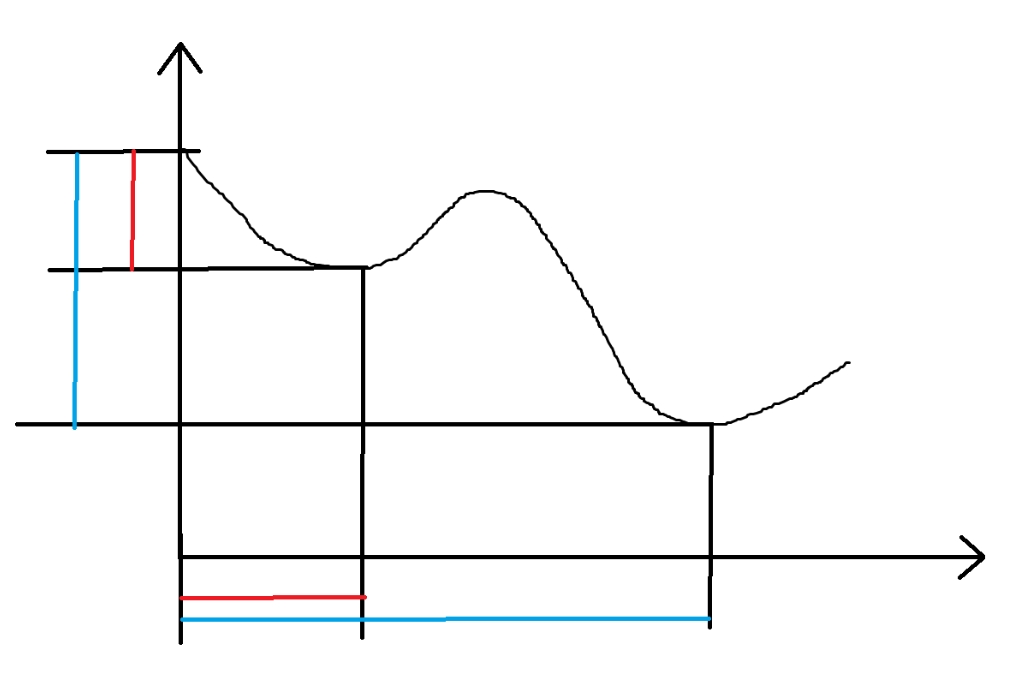
\includegraphics[width=0.35\textwidth]{./image/22.png}
    \caption{最速下降步长}
    \label{fig:Chapter4_Temporary_Pavilion_1}
\end{figure}
实际上,读者可能会想到,如果我们每次都要实时计算步长,岂不是降低了效率吗?这个问题是有道理的,请看下面的流程图:
\begin{figure}[H]
    \centering
    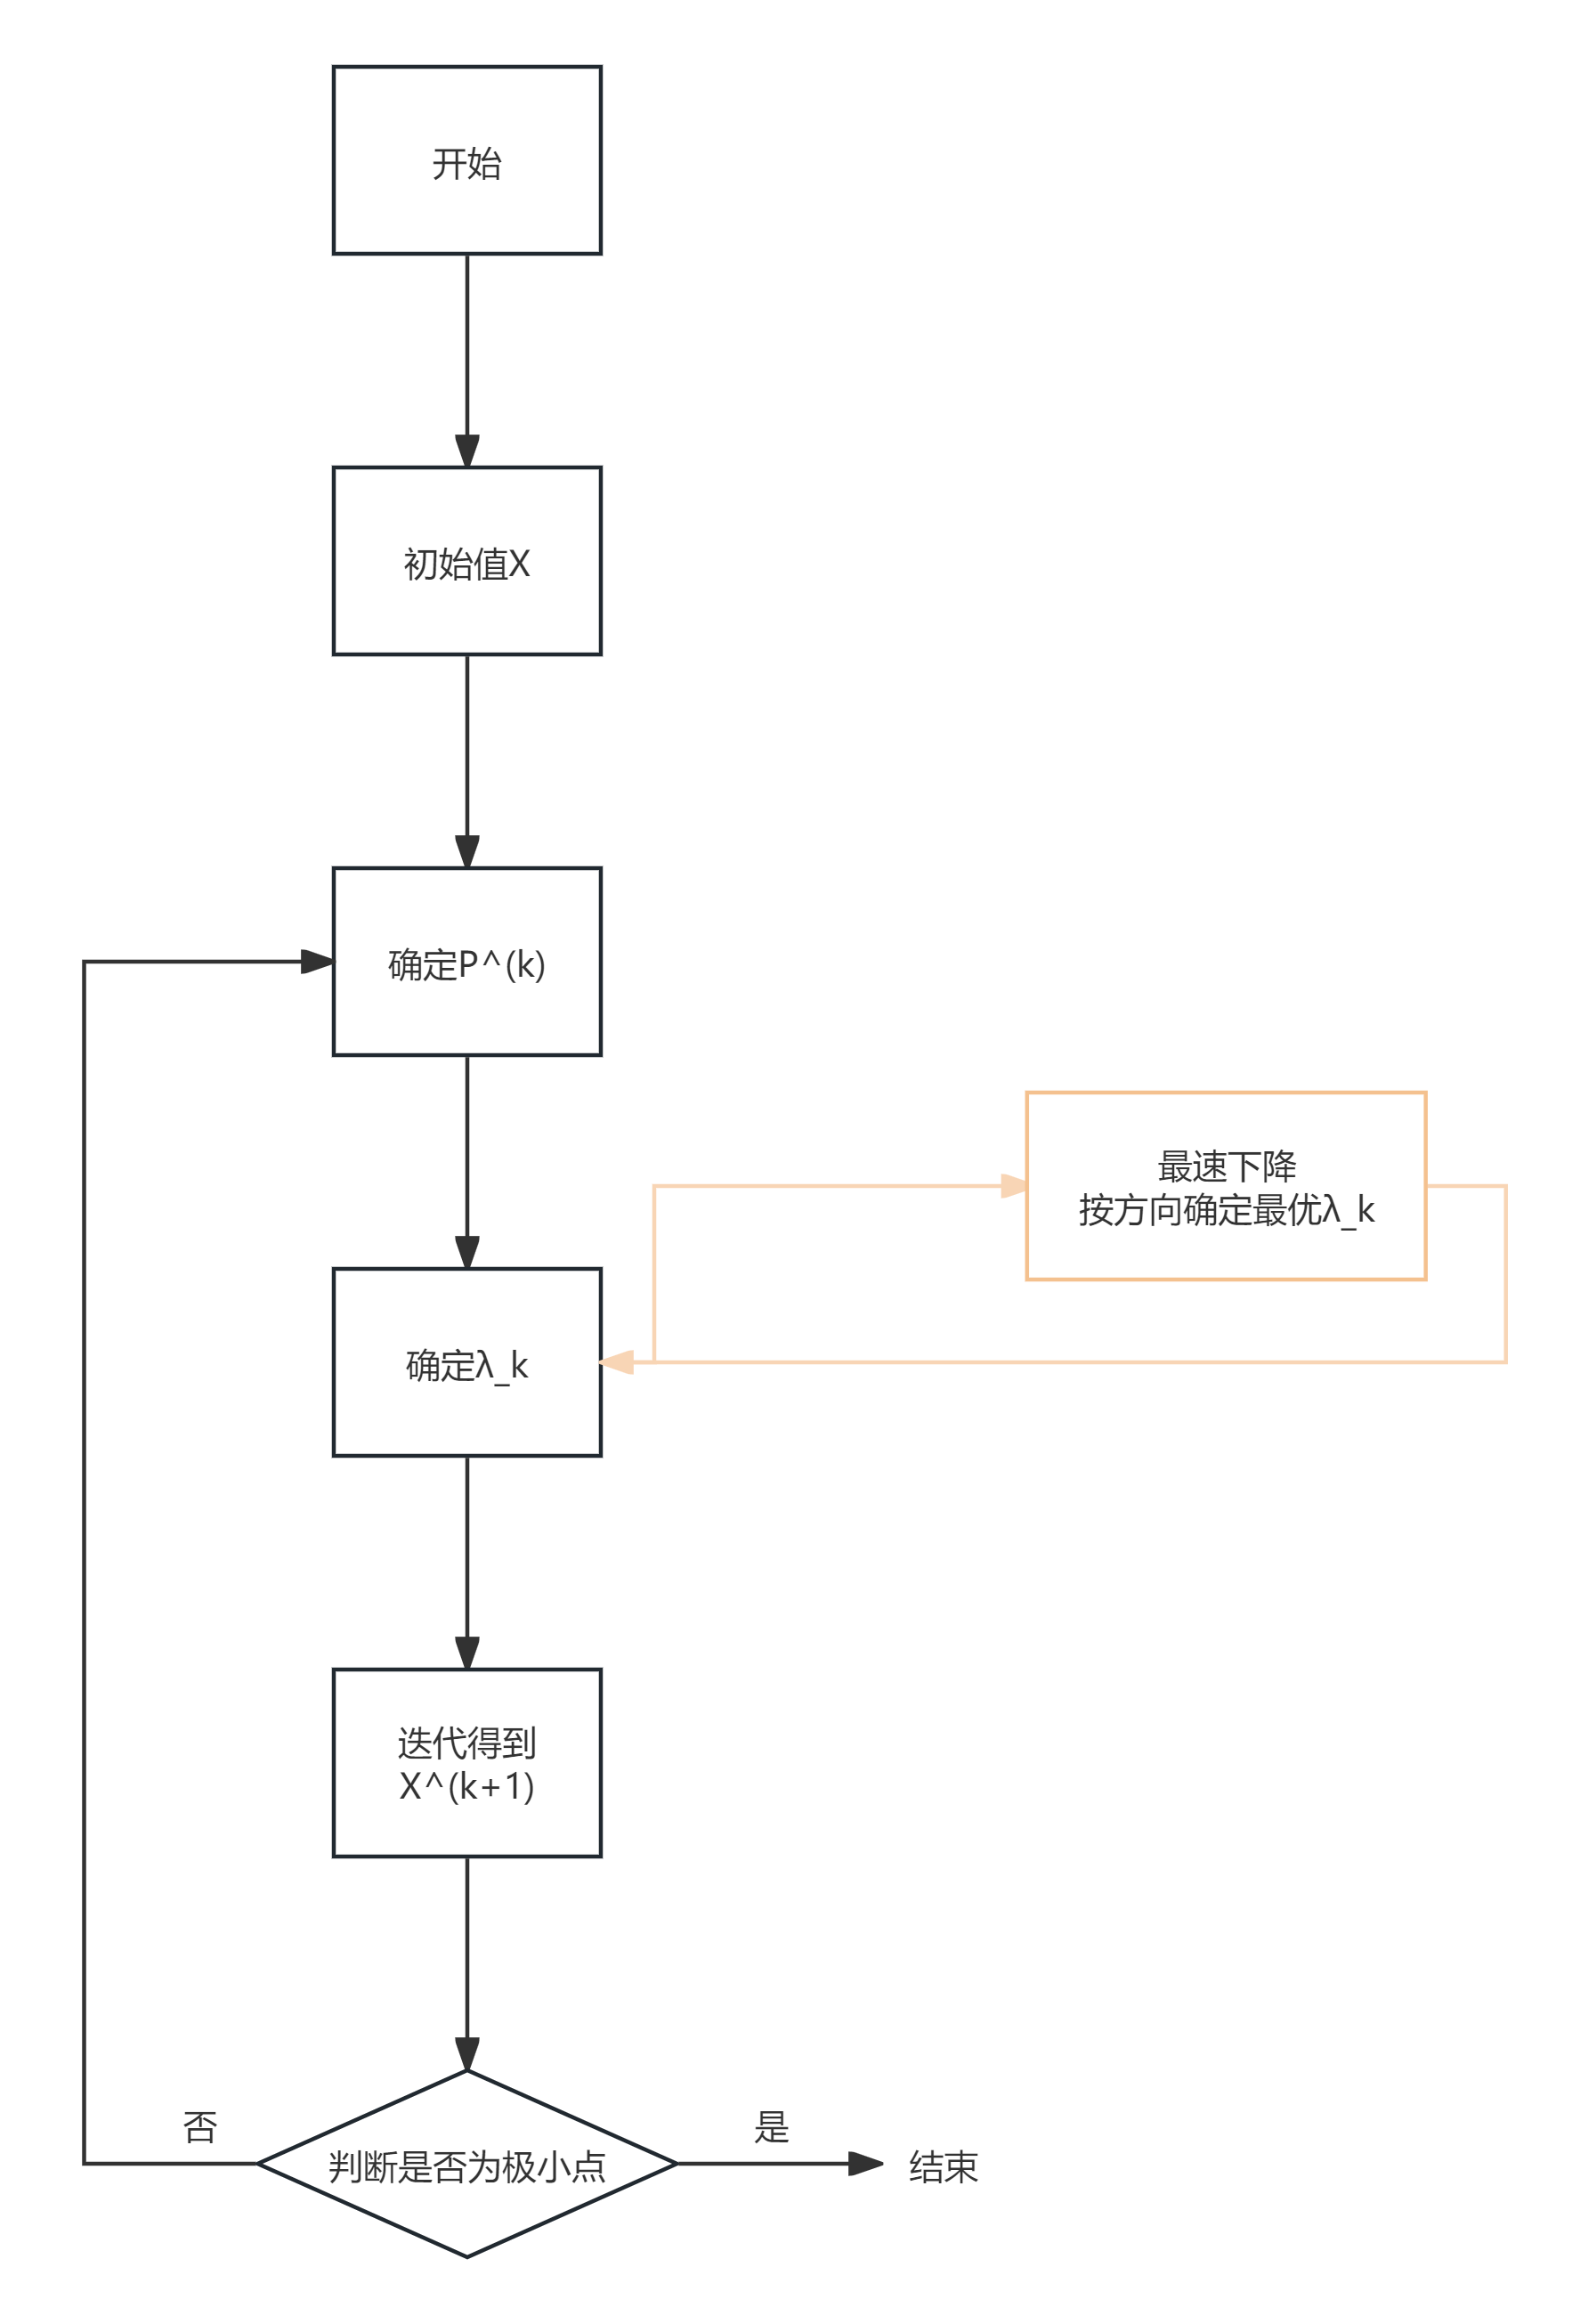
\includegraphics[width=0.6\textwidth]{./image/23.png}
    \caption{流程图}
    \label{fig:Chapter4_Temporary_Pavilion_1}
\end{figure}
引入\textcolor{orange}{橙色环节}之前,可能需要迭代100次,每次执行1秒;引入橙色环节之后,可能需要迭代50次,每次执行2秒。所以总的时间谁多谁少很难说了。因此我们想到,是否有办法在迭代过程中,既能带有最优步长的色彩,计算又不过于复杂?
\subsubsection{确定迭代步长的黄金分割法(0.618法)}
\label{确定迭代步长的黄金分割法}
\begin{notebox}{\textbf{黄金分割法(0.618 法)}}{}
    \\作为一种计算更简便的方法,黄金分割法在区间缩短效率上近似斐波那契法。
    \[
    x_k' = a_{k-1} + 0.382 [b_{k-1} - a_{k-1}]
    \]
    \[
    x_k'' = a_{k-1} + 0.618 [b_{k-1} - a_{k-1}]
    \]
    其中 $x_k'$ 和 $x_k''$ 分别是 $[a_{k-1}, b_{k-1}]$ 区间内的两个点,$0.382$ 和 $0.618$ 是黄金分割法的两个常数。
    可以这么理解:$x_k'$其实是$a_k$,$x_k''$其实是$b_k$,新的$\lambda_k$为$b_{k}-a_{k}$,旧的$\lambda_{k-1}$为$a_{k-1}-b_{k-1}$ 
\end{notebox}
总结一下,为了理清楚框架,我们通过本节学习了以下内容:
\begin{enumerate}
    \item \textbf{非线性规划问题的定义}
    
    \item \textbf{非线性规划问题的数学模型(模型 I 与模型 II 的转换)}
    \begin{itemize}
        \item 一般形式
        \item 标准模型 I
        \item 标准模型 II
    \end{itemize}
    
    \item \textbf{求解非线性规划问题的方法}
    \begin{itemize}
        \item \textbf{解析法}
        \begin{itemize}
            \item 前置概念:梯度、平稳点、Hesse矩阵、正定矩阵
            \item 定理一:极值点必要条件
            \item 定理二:局部极值点判断的充要条件
        \end{itemize}
        
        \item \textbf{数值法(下降迭代算法)}
        \begin{enumerate}
            \item 初值的确定
            \item 算法的设计
            \begin{enumerate}
                \item 步长的确定
                \begin{itemize}
                    \item 恒定步长
                    \item 变步长
                    \item 最速下降步长
                    \begin{enumerate}
                        \item 一维搜索
                        \item 黄金分割法
                    \end{enumerate}
                \end{itemize}
                \item 搜索方向的确定(更为重要,后面介绍)
            \end{enumerate}
            \item 算法的结束条件
        \end{enumerate}
    \end{itemize}
\end{enumerate}


\section{无约束非线性规划问题的解}
\begin{thmbox}{无约束非线性规划}{cool}
$$
\min f(X) 
$$
\end{thmbox}
接下来介绍无约束非线性规划的几个解决办法。关键要点是确定下降的方向$P^{(k)}$,步长的计算还是用之前的内容。
\subsection{梯度法(最速下降法)}

\begin{notebox}{\textbf{梯度法(最速下降法)}}{}\\
    \noindent 一般性的数值法方式为

    \[
    X^{(k+1)} = X^{(k)} + \lambda_k P^{(k)} \quad \lambda_k \geq 0
    \]

    \bigskip
    \noindent $X^{(k)}$ ——— 第 $k$ 步迭代结果

    \bigskip
    \noindent $X^{(k+1)}$ ——— 将要进行的第 $k+1$ 步迭代点

    \bigskip
    \noindent $\lambda_k$ ——— 第 $k$ 步已迭代完成的情况下,下一步的迭代步长

    \bigskip
    \noindent $P^{(k)}$ ——— 第 $k$ 步已迭代完成的情况下,下一步的搜索方向

    \bigskip
    \noindent \textbf{每次迭代的目标}:使目标函数数值每次都有所下降,即:

    \[
    f(X^{(k+1)}) < f(X^{(k)})
    \]
    且我们希望下降的最多。
\end{notebox}
我们采用的方法如下\footnote{说人话,就是每到新的一处后算出来梯度后反着下降,到下一处再算梯度,以此类推;读者可以想到这种方法虽然提升了每次下降最快的效率,但是对于全局的效率来说未必是好的——每次下降仅考虑当前点如何最快,类似于贪心算法}:
\begin{enumerate}
    \item 为此目标,考察 $f(X)$ 在 $X^{(k)}$ 点的泰勒级数(即在 $X^{(k)}$ 对 $f(X)$ 展开):
    \[
    f(X^{(k+1)}) = f(X^{(k)} + \lambda_k P^{(k)}) \quad \text{(由一维迭代公式)}
    \]
    \[
    = f(X^{(k)}) + \lambda_k \nabla f^T(X^{(k)}) P^{(k)} + o(\lambda_k),
    \]
    \[
    \therefore \text{只要满足上式中间项一项 } \lambda_k \nabla f^T(X^{(k)}) P^{(k)} < 0 \text{,目标函数就是下降的,即 }\\
     f(X^{(k+1)}) < f(X^{(k)})
    \]
    
    \item 进一步,如果希望 $f(X^{(k+1)})$ 在 $f(X^{(k)})$ 的基础上下降的最多,则合适的 $P^{(k)}$,
    
    使泰勒展开式中间项一项 $\lambda_k \nabla f^T(X^{(k)}) P^{(k)}$ 取最大负值(此时假设 $\lambda_k$ 已选定),

    为此:
    \[
    \because \lambda_k > 0 \quad \therefore \lambda_k \nabla f^T(X^{(k)}) P^{(k)} < 0 \Rightarrow \nabla f^T(X^{(k)}) P^{(k)} < 0,
    \]

    对于 $\nabla f^T(X^{(k)}) P^{(k)} < 0$ 来说,$\nabla f^T(X^{(k)})$ 和 $P^{(k)}$ 是两个向量(且前者已确定),

    由几何学原理知道,当两个矢量大小相同,方向相反,其点积取最大负值:
    \[
    \therefore \text{取 } P^{(k)} = -\nabla f^T(X^{(k)}),
    \]
    \[
    \therefore \nabla f^T(X^{(k)}) P^{(k)} = -\nabla f^T(X^{(k)}) \cdot \nabla f(X^{(k)}) = -\|\nabla f^T(X^{(k)})\|^2 < 0,
    \]

    即为负值,又数值最小,

    \[
    \therefore \text{当取 } P^{(k)} = -\nabla f^T(X^{(k)}) \text{ 时,} f(X^{(k+1)}) \text{ 比 } f(X^{(k)}) \text{ 下降的最多,}
    \]
    
    \noindent ——称为负梯度方向。
    \item 得到了搜索方向 $P^{(k)}$,再用一维搜索进一步求取最佳的步长 $\lambda_k$,即:\\
    \[
    \text{负梯度搜索方向} + \text{一维搜索步长} \quad \Rightarrow \quad \text{最速下降法}
    \]
\end{enumerate}

\begin{notebox}{\textbf{迭代求解过程:}}{}
\\
    \noindent \textbf{Step 1:} 给定初始迭代点 $X^{(0)}$ 及容许精度 $\varepsilon > 0$,

    \bigskip
    \noindent 若 $\|\nabla f^T(X^{(0)})\|^2 \leq \varepsilon$,则 $X^{(0)}$ 即为近似最优解,停止迭代,

    \bigskip
    \noindent \textbf{Step 2:} 若 $\|\nabla f^T(X^{(0)})\|^2 > \varepsilon$,求步长 $\lambda_0$,并计算 $X^{(1)} = X^{(0)} - \lambda_0 \nabla f(X^{(0)})$,

    \bigskip
    \noindent \textbf{Step 3:} 当迭代到第 $k$ 步后,

    \bigskip
    \noindent 若 $\|\nabla f^T(X^{(k)})\|^2 < \varepsilon$,则 $X^{(k)}$ 即为近似最优解,

    \bigskip
    \noindent 否则,则确定下一个迭代点 $X^{(k+1)}$ 为,
    \[
    X^{(k+1)} = X^{(k)} - \lambda_k \nabla f(X^{(k)}),
    \]

    \noindent 并通过黄金分割法求最优的 $\lambda_k$。
\end{notebox}
    

\subsection{共轭梯度法}
这一方法主要解决的是正定二次函数最小问题,用代数的方法理解,我们知道任意非线性函数都可以由泰勒展开,用多项式无穷地逼近,
可以近似到最高阶次;同理,理论上所有的非线性规划问题都可以近似成正定二次函数最小问题。接下来我们就了解共轭、正定二
次函数最小问题的概念,以及在此基础上提出的共轭方向法,指出其不足,并了解在其基础上改进而成的共轭梯度法。\\
\begin{dfnbox}{正交与共轭}{amznotes}
    \begin{enumerate}
        \item 若 $X \in R^n, Y \in R^n$,当 $X^T Y = 0$ 时,称 $X$ 与 $Y$ 正交。
        
        \item 若 $A$ 为 $n \times n$ 对称正定矩阵,当 $X^T A Y = 0$ 时,称 $X$ 和 $Y$ 关于 $A$ 共轭,或 $X$ 和 $Y$ 为 $A$ 共轭。
        
        当 $A$ 为单位矩阵时,即为 $X$ 和 $Y$ 正交,所以\textbf{正交是共轭的一种特殊情况}。
        
        \item 若 $A$ 为 $n \times n$ 对称正定矩阵,若非零向量 $P^{(0)}, P^{(1)}, \cdots, P^{(n)} \in R^n$,关于 $A$ 两两共轭,即:
        \[
        (P^{(i)})^T A (P^{(j)}) = 0, \quad i \neq j, \quad i, j = 1, 2, \cdots, n
        \]
        则称向量组为 $A$ 共轭。
    \end{enumerate}
\end{dfnbox}
\begin{thmbox}{关于 $A$ 共轭的向量组线性无关}{cool}
    关于 $A$ 共轭的向量组线性无关。
\end{thmbox}
\begin{dfnbox}{正定二次函数最小问题}{amznotes}
    无约束极值取值问题的一个特殊情况是:
    \[
    \min f(X) = \frac{1}{2} X^T A X + B^T X + C,
    \]
    其中:$A$ 为 $n \times n$ 对称正定矩阵,$B$ 为系数向量,$C$ 为常数,

    \noindent —— 称为\textbf{正定二次函数最小问题}。
\end{dfnbox}
\begin{thmbox}{共轭方向法}{cool}
    设向量 $P^{(i)}, \ i=0,1,2,\cdots,n-1$ 为 $A$ 共轭,则从任一点 $X^{(0)}$ 出发,相继以
    \[
    P^{(0)}, P^{(1)}, \cdots, P^{(n-1)}
    \]
    为搜索方向的迭代算法:

    \[
    \begin{cases}
        \min f(X^{(k)} + \lambda P^{(k)}) = f(X^{(k)} + \lambda_k P^{(k)}), \\
        X^{(k+1)} = X^{(k)} + \lambda_k P^{(k)}
    \end{cases}
    \]

    经 $n$ 次迭代后就能收敛于正定二次函数最小问题的极值解,

    \noindent —— 称为\textbf{共轭方向法}。
\end{thmbox}
一般来说,共轭方向法仅具有理论分析意义,对于实际的正定二次函数极小问题求解,共轭方向法至少有二方面问题没有解决:
\begin{enumerate}
    \item A 共轭的搜索方向向量组理论上为\[
    P^{(0)}, P^{(1)}, \cdots, P^{(n-1)}
    \]
    但实用时如何构造这n个向量,它们具有什么形式,没有说明。
    \item 尽管在理论上只需n次迭代就能命中目标,但实际的运算误差的存在,使问题的解具有不定性。
\end{enumerate}
其中,第一点是致命的,使共轭方向法不具备可操作性。为此,发展了共轭方向法的一种具体算法——\textbf{共轭梯度法}。
\\其主要特点是: 基于梯度,构造了一组可实现的共轭方向,使算法具有可操作性。共轭梯度法是一种构造性方法。

\begin{notebox}{\textbf{非正定二次函数的共轭梯度法}}{}
    \\对于更广泛的一般无约束非线性规划,
    \[
    \min f(X),
    \]

    \noindent 可以通过逼近当前迭代点附近是够小的邻域内进行泰勒级数近似的方式,将一般非线性函数展开成二次函数,而采用具有一定迭代精度的共轭梯度法。

    \[
    f(X^{(k+1)}) = f(X^{(k)} + \lambda_k P^{(k)}),
    \]

    \[
    \approx f(X^{(k)}) + \lambda_k f^T(X^{(k)}) P^{(k)} + \frac{1}{2} \lambda_k^2 (P^{(k)})^T H(X^{(k)}) P^{(k)},
    \]

    \noindent “$\approx$”右边是二次函数。
\end{notebox}
读者可以这样理解这一方法:不同于5.1.1节,每次迭代后方向都根据梯度来进行调整,共轭梯度法是先根据梯度确定了$P^{(0)}$,再用其构建与其共轭的$P^{(1)}$,根据$P^{(1)}AP^{(0)}=0$,其中$A$和$P^{(0)}$均已知,解方程即可;之后再确定$P^{(2)}$,要求其与$P^{(0)}$和$P^{(1)}$均共轭,依次类推。\\

\subsection{变尺度法}
在前述梯度法和共轭梯度法中,确定搜索方向时充分利用了目标函数的梯度信息。假若目标函数的二阶导数信息(Hesse矩阵)也存在,我们就有理由利用二阶导数信息确定搜索方向。
\begin{notebox}{\textbf{广义牛顿法}}{}
    \\

    一种可能是,采用
    
    \[
    P^{(k)} = -H(X^{(k)})^{-1} \nabla f(X^{(k)}) 
    \]
    作为搜索方向,
    
    即
    
    \[
    X^{(k+1)} = X^{(k)} + \lambda_k P^{(k)}
    \]
    
    \[
    P^{(k)} = -H(X^{(k)})^{-1} \nabla f(X^{(k)}), \quad \lambda_k = \min_\lambda f(X^{(k)} + \lambda P^{(k)})
    \]
    称为\textbf{广义牛顿法}。
    
    \[
    P^{(k)} = -H(X^{(k)})^{-1} \nabla f(X^{(k)}) 
    \]
    称为$f(X)$在$X^{(k)}$的牛顿方向。
\end{notebox}
广义牛顿法是一个相当优秀的算法,但在应用时求 Hesse 矩阵的逆很麻烦。为了不计算 Hesse 矩阵(从而不必计算 Hesse 逆),通过构造一个近似于 Hesse矩阵的逆矩阵来满足迭代要求。
称为\textbf{变尺度法}。
\\下面来讨论如何构造$H(X^{(k)})$一的近似矩阵$\overline{H^{(k)}}$。为此,提出以下要求:
\begin{enumerate}
    \item 每做一次迭代,目标函数应下降。
    \item 每一步都能用现有信息确定下一个搜索方向。
    \item 这些近似矩阵最后应收敛于解点处的 Hesse 矩阵的逆。
\end{enumerate}

\section{约束非线性规划问题(约束极值问题)}
\begin{thmbox}{约束非线性规划}{cool}
\[
\min f(x)
\]

\[
h_i(x) = 0, \quad i = 1, 2, \dots, m
\]

\[
g_j(x) \geq 0, \quad j = 1, 2, \dots, l
\]
或

\[
\min f(x)
\]

\[
g_j(x) \geq 0, \quad j = 1, 2, \dots, l
\]

\[\because
\quad h_l(x) = 0 \iff
\begin{cases}
h_l(x) \geq 0 \\
h_l(x) \leq 0
\end{cases}
\]

\[\therefore
\text{统一采用后一形式。}
\]

若采用集合形式,则为:

\[
\min f(x), \quad x \in K \subset \mathbb{R}^n
\]

\[
K = \{x \mid g_j(x) \geq 0, \quad j = 1, 2, \dots, l\}
\]
\end{thmbox}
求解约束极值问题要注意以下两点(原则):
\begin{itemize}
    \item 目标函数在每次迭代都有所下降(涉及目标函数)
    \item 解的可行性问题,即解要在可行域中(涉及约束条件)
\end{itemize}
求解约束极值问题的三种主要思路:
\begin{enumerate}
    \item \textbf{将迭代点严格局限于可行域内},将迭代点序列严格控制在可行域内,从而执行的迭代过程实际上为无约束优化过程。例如:
    \begin{itemize}
    \item \textbf{数值法}中的\hyperref[sec:可行方向法]{可行方向法}
    \end{itemize}
    \item \textbf{约束极值问题化为无约束问题},序列无约束优化方法,简称SUMT方法,又称制约函数法。该方法通过将约束项处理成制约函数项加入到目标函数中形成新的广义目标函数,从而将有约束问题化为广义目标函数下的无约束问题,再利用前述的无约束优化迭代算法求解。例如:
    \begin{itemize}
        \item \textbf{解析法}中的拉格朗日乘子法、\hyperref[sec:K-T条件]{K-T条件}
        \item \textbf{数值法}中的\hyperref[sec:制约函数法]{制约函数法},包括惩罚函数(内点法)和障碍函数(外点法)。
    \end{itemize}
    \item \textbf{复杂约束极值问题化为简单约束问题},在迭代点附近的序列线性化或序列二次函数逼近方法,通过运用迭代点附近的台劳展开,将有约束的非线性规划近似为极易求解的线性规划或二次
    规化以实现迭代求解。例如:
    \begin{itemize}
        \item \textbf{数值法}中的\hyperref[sec:逐次逼近类方法]{逐次逼近类方法},包括逐次线性规划法(SLP)和逐次二次规划法(SQP)。
    \end{itemize}

\end{enumerate}

\subsection{解析法:K-T条件}
\label{sec:K-T条件}
拉格朗日乘子法是将约束极值问题化为无约束问题的一种方法。\\
\begin{notebox}\textbf{{拉格朗日乘子法}}{}
\\对于约束条件是等式的问题,例如:
$$
\min f(x)
$$
$$
s.t. g(x)=0
$$
我们可以将其转化为:
$$
\min F(x)=f(x) + \lambda g(x)\\
$$
这样就变成了无约束的极值问题。
\end{notebox}
那么对于不等式约束条件的情况,这一思想是否还适用呢?答案是肯定的。\\
前已述及,非线性规划问题一般难以用解析法求解。然而,经过多年的研究,还是得到了许多可以用于解析求解的理论成果,库恩-塔克条件就是其中最重要的一个。
\begin{dfnbox}{K-T条件}{}
设 $x^*$ 是非线性规划:

\[
\min f(x)
\]

\[
g_j(x) \geq 0, \quad j = 1, 2, \dots, l
\]
的局部极小点,$f(x)$ 和 $g_j(x)$, $j = 1, 2, \dots, l$ 在点 $x^*$ 有一阶连续偏导数,而且在 $x^*$ 处所有起作用的梯度线性无关,则存在数 $\mu_1^*, \mu_2^*, \dots, \mu_l^*$ 使得:

\[
\nabla f(x^*) - \sum_{j=1}^{l} \mu_j^* \nabla g_j(x^*) = 0
\]

\[
\mu_j^* g_j(x^*) = 0, \quad j = 1, 2, \dots, l
\]

\[
\mu_j^* \geq 0
\]

以上称为\textbf{卡恩—塔克条件(K-T 条件)},满足该条件的点称为\textbf{卡恩—塔克点},$\mu_1^*, \mu_2^*, \dots, \mu_l^*$ 称为\textbf{拉格朗日(Lagrange)乘子}。
\end{dfnbox}
对此我们有四点说明:
\begin{enumerate}
    \item K-T条件为必要条件,只要x是极值点,且起作用约束的梯度线性无关,则该条件就成立。
    \item 满足K-T 条件的并非一定是最优点。
    \item 对于凸规划\footnote{凸规划是特别简单、特别特殊的一类,但是我们常见的问题都不属于凸规划,因此不用深究},K-T条件不但是必要条件,而且是充分条件。
    \item 得到的库恩塔克点须代入到约束条件$g_j(x)\geq0,j=1,2,\cdots,l$中验证是否满足。
\end{enumerate}
\begin{exbox}{用K-T条件求解非线性规划}{}
\textbf{例:}若有
$$
\max f(x)=(x-4)^2
$$
$$
1\leq x \leq 6
$$
\textbf{解:} 变为标准形式:

\[
\min \ f(x) = -(x-4)^2
\]
约束条件为:

\[
g_1(x) = x - 1 \geq 0, \quad g_2(x) = 6 - x \geq 0
\]
对应梯度:

\[
\nabla f(x) = -2(x - 4), \quad \nabla g_1(x) = 1, \quad \nabla g_2(x) = -1
\]
设K-T点为 \( x^* \),对两个约束条件引入拉格朗日乘子 \( \mu_1, \mu_2 \),得到K-T条件:

\[
-2(x^* - 4) - \mu_1 + \mu_2 = 0
\]

\[
\mu_1 (x^* - 1) = 0
\]

\[
\mu_2 (6 - x^*) = 0
\]

\[
\mu_1 \geq 0, \ \mu_2 \geq 0
\]

解以上方程组,得到:
\begin{itemize}
    \item (1) \( \mu_1 > 0, \ \mu_2 > 0 \), 无解
    \item (2) \( \mu_1 > 0, \ \mu_2 = 0 \), \( x^* = 1, f(x^*) = 9 \)
    \item (3) \( \mu_1 = 0, \ \mu_2 = 0 \), \( x^* = 4, f(x^*) = 0 \)
    \item (4) \( \mu_1 = 0, \ \mu_2 > 0 \), \( x^* = 6, f(x^*) = 4 \)
\end{itemize}

\textbf{结论:} 三个K-T点 \( x^* = 1, \ x^* = 4, \ x^* = 6 \),经验证 \( 1 \leq x \leq 6 \),都在可行域内。最大点为 \( x^* = 1, f(x^*) = 9 \),最小点为 \( x^* = 4, f(x^*) = 0 \)。
\end{exbox}


\subsection{数值法:可行方向法}
\label{sec:可行方向法}
考虑最小化问题:

\[
\min f(x)
\]
约束条件:

\[
g_j(x) \geq 0, \quad j = 1, 2, \dots, l
\]

设 \( x^{(k)} \) 是第 \( k \) 步可行解,则第 \( k+1 \) 步可行解为:

\[
x^{(k+1)} = x^{(k)} + \lambda_k D^{(k)} \in K
\]
其中,\( f(x^{(k+1)}) < f(x^{(k)}) \),且 \( \lambda_k \) 为步长,\( D^{(k)} \) 为某一可行方向\footnote{和无约束相比,仅仅把P变成D了,就是可行方向}。

\begin{dfnbox}{可行方向法}{}
    所谓可行方向法,是指具有以下特点的一类数值迭代算法:
    \begin{itemize}
        \item 若满足迭代精度要求。
        \[
        \|x^{(k-1)} - x^{(k)}\| < \varepsilon_1
        \]
        \[
        |f(x^{(k-1)}) - f(x^{(k)})| < \varepsilon_2
        \]
        则停止迭代,找到了近似最优解。
        
        \item 若不满足精度要求,则继续沿可行方向迭代,直到满足要求。
    \end{itemize}
\end{dfnbox}
可行方向法具有三个特点:
    \begin{enumerate}
        \item 搜索方向为可行方向。
        \item 迭代点序列始终在可行域内。
        \item 目标函数值单调下降。
    \end{enumerate}
可以说,约束极值问题的大多数数值迭代算法具有可行方向法的特点,所以很多方法都可以归入可行方向法这一类。但是,我们通常所说的可行方向法,是指 Zoutendijk 于 1960 年提出的算法及其变形。
\\\textbf{说明:}
    
在以前的算法中,搜索方向直接通过设置来确定,例如:
\begin{enumerate}
    \item 直接设置为负梯度方向——最速下降法。
    \item 直接设置为牛顿方向——牛顿法、拟牛顿法、变尺度法。
    \item 直接改为共轭方向——共轭方向法、共轭梯度法。
    \item ……
\end{enumerate}
这种直接设置的方法代表了一大类算法。\\
可行方向法的思想与直接设置的方法不同,它是通过一种 \(n\) 维线性寻优的方法求取一个最优的搜索方向,从理论上说更完美。
\\\textbf{思路:}\\
\begin{itemize}
    \item 一个方程确保下降(只跟目标函数有关),另一个方程确保可行(只跟约束条件有关),关联点就是可行方向$D$;
    \item 为了保证保险,设置一个系数$\eta<0$使得在迭代的过程中更不敏感;在此基础上用线性规划寻找最优的$\eta$
\end{itemize}
\begin{notebox}{\textbf{Zoutendijk 可行方向法}}{}
    \begin{itemize}
    \item \textbf{Zoutendijk 可行方向法:}\\
    设 \( X^{(k)} \) 点的起作用约束集非空,为求 \( X^{(k)} \) 点的可行下降方向,可通过以下条件\footnote{第一个条件是之前提到过的向量内积为负,即解决的是下降问题;第二个条件是保证可行的问题}:
    \[
    \begin{cases}
        \nabla f^T \left( X^{(k)} \right) D < 0, \\
        \nabla g_j \left( X^{(k)} \right) D > 0 & j \in J.
    \end{cases}
    \]
    
    令 \(\eta < 0\),则上述式化为更严格条件\footnote{想象一个在可行域边界的点,如果没有$\eta$,那么根据条件2,下降的方向就是从这一点出发向可行域内的任何方向,但是不能向外出了可行域;有了$\eta$,那么下降的方向会进一步收缩,$\eta$绝对值越大,收缩的程度越大}:
    \[
    \begin{cases}
        \nabla f^T \left( X^{(k)} \right) D \leq \eta, \\
        -\nabla g_j \left( X^{(k)} \right) D \leq \eta & j \in J.
    \end{cases}
    \]
    其中 \(\eta < 0\)。

    \item \textbf{最佳可行方向的求解:}
    
    为寻求一个最佳的可行方向(如目标函数下降最多的可行方向),对
    \[
    \nabla f^T \left( X^{(k)} \right) D \leq \eta \text{ 和 } \nabla g_j \left( X^{(k)} \right) D \leq \eta \quad (j \in J)
    \]
    沿 \(\eta\) 极小化,即:
    
    将“选取最佳可行方向问题”转化为对 \(\eta\) 的线性规划问题:
    \[
    \begin{aligned}
        & \min_D \eta \\
        & \text{s.t.} \quad \nabla f^T \left( X^{(k)} \right) D \leq \eta, \\
        & \qquad -\nabla g_j \left( X^{(k)} \right) D \leq \eta \quad (j \in J), \\
        & \qquad -1 \leq d_i \leq 1 \quad (i = 1, 2, \dots, n).
    \end{aligned}
    \]
    其中 \(d_i\) 为 \(D\) 的第 \(i\) 个分量,约束 \(-1 \leq d_i \leq 1\) 用于限制 \(D\) 的大小。
\end{itemize}
\end{notebox}
 
\subsection{数值法:制约函数法}
\label{sec:制约函数法}
序列无约束优化方法中常用的制约函数基本上有两类,一类为\textbf{罚函数},又称为\textbf{外点法}\footnote{这种方法允许跑到可行域外,但是会施加惩罚,就像是开放世界冒险游戏,跑到地图外边扣血,逼着你回去!};一类为\textbf{障碍函数},又称为\textbf{内点法}\footnote{这是在可行域边界设立“障碍”,让你跑不出去,就相当于开放世界冒险游戏里的空气墙!}。
\subsubsection{外点法}
\begin{notebox}{\textbf{惩罚函数法}}{}
    \begin{itemize}
    \item \textbf{求解思路}
    \\考虑约束非线性规划的原问题:
    \[
    \min f(x), \quad x \in R = \{ x \mid g_j(x) \geq 0, \, j = 1, 2, \ldots, l \}.
    \]
    
    若能构造一个关于 \( g_j(x) \) 的函数 \(\psi(g_j(x))\),满足:
    \[
    \psi(g_j(x)) = 
    \begin{cases} 
        0 & x \in R, \\ 
        \infty & x \notin R,
    \end{cases}
    \]
    则可将约束极值问题转化为无约束极值问题。
    \item \textbf{复合函数的构造}

    令 \(\psi(g_j(x)) \to \psi(x)\),并定义:
    \[
    \Phi(x) = f(x) + \sum_{j=1}^l \psi(g_j(x)).
    \]
    此时,原问题的约束非线性规划可通过 \(\Phi(x)\) 化为无约束非线性规划:
    \[
    \min f(x), \quad x \in R \quad \Rightarrow \quad \min \Phi(x).
    \]
\end{itemize}
\end{notebox}
\begin{figure}[H]
    \centering
    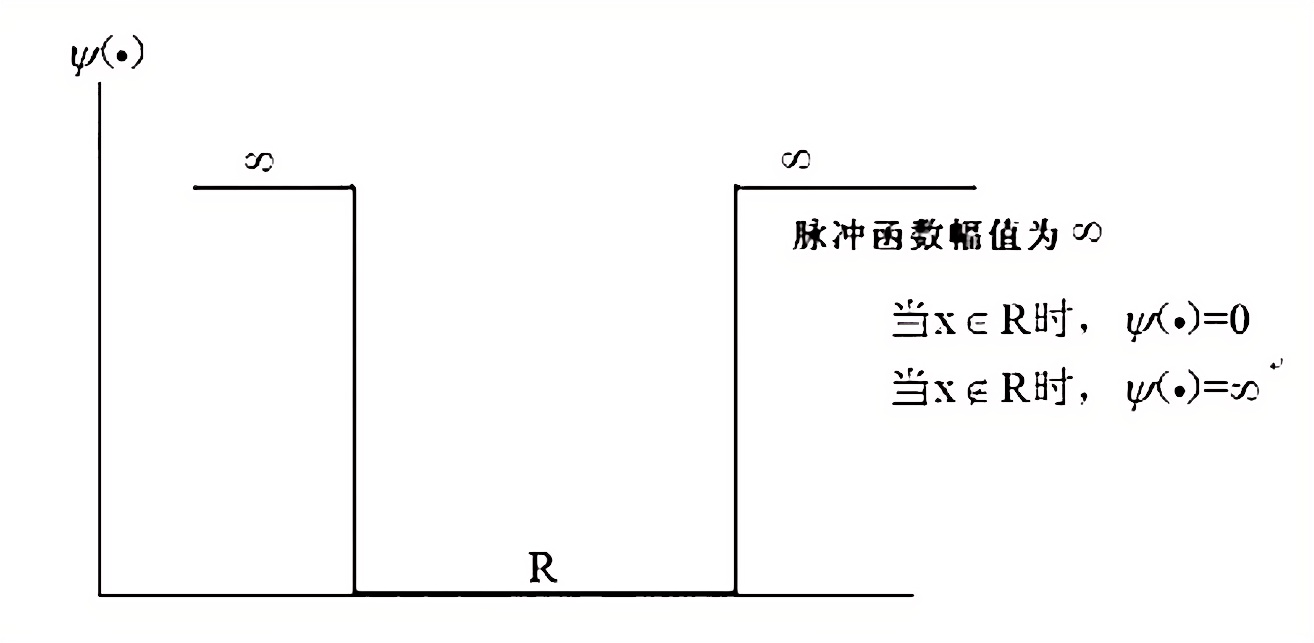
\includegraphics[width=0.5\textwidth]{./image/24.png}
    \caption{理想的罚函数}
    \label{fig:Chapter4_Temporary_Pavilion_1}
\end{figure}
\begin{thmbox}{等价性验证}{}
\textbf{等价性验证}
    \begin{enumerate}
        \item 当 \( x \in R \) 时,\(\min \Phi(x) = \min f(x) + 0 = \min f(x)\)。
        \item 当 \( x \notin R \) 时,\(\min \Phi(x) = \infty\) 无解。
    \end{enumerate}
因此,原问题的求解等价于:
    \[
    \min \Phi(x).
    \]
\end{thmbox}
    \textbf{脉冲函数的改进}

    由于脉冲函数 \(\psi(\cdot)\) 在边界上不连续且难以实现,将其改进为具有更好可实现性和光滑性的函数:
    \[
    \psi(g_j(x)) = [\min(0, g_j(x))]^2 = 
    \begin{cases} 
        0 & x \in R, \\ 
        (g_j(x))^2 & x \notin R.
    \end{cases}
    \]
    在 \( x \notin R \) 处,函数具有二次形式的特点,如下图:
    \begin{figure}[H]
        \centering
        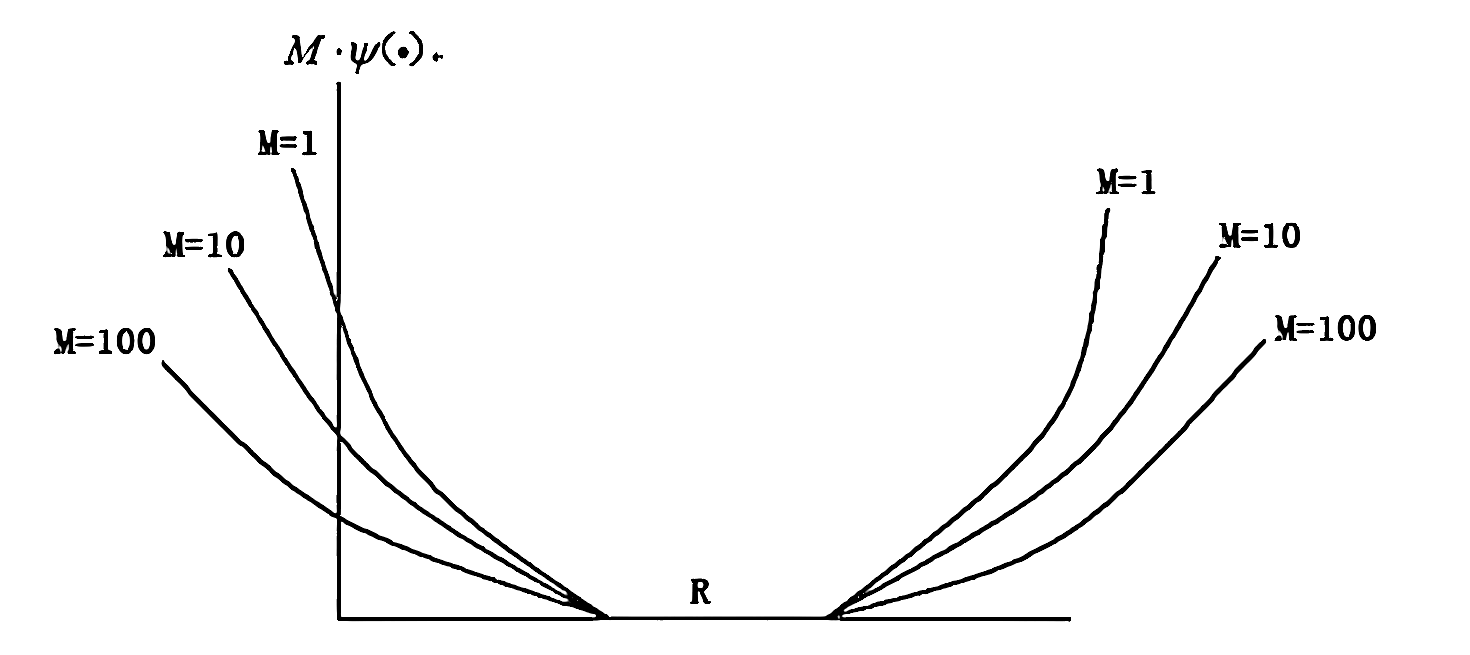
\includegraphics[width=0.5\textwidth]{./image/25.png}
        \caption{改进的罚函数}
        \label{fig:Chapter4_Temporary_Pavilion_1}
    \end{figure}
    \begin{notebox}{\textbf{目标函数的构造}}{}
    \\取一个充分大的正数 \( M > 0 \),构造新的目标函数:
    \[
    P(x, M) = f(x) + M \sum_{j=1}^{l} \psi(g_j(x)) = f(x) + M \sum_{j=1}^{l} [\min(0, g_j(x))]^2.
    \]
    此时,求解:
    \[
    \min P(x, M)
    \]
    与原问题等价。式中,\( P(x, M) \) 称为惩罚函数,第二项称为惩罚项,\( M \) 称为惩罚因子。
    \end{notebox}
    总之,不同于之前的方法,该方法允许“跑到可行域外”,但是,代价是什么呢?那就是惩罚函数。几点说明:
    \begin{enumerate}
    \item 首先
    \begin{itemize}
        \item 若$X$在$R$内,则$P(x,M)$变为无约束非线性规划问题;
        \item 若$X$在$R$外,即$XR$,则$X$离$R$越远,惩罚项越大,促使下一步的选代点拉向$R$内。 
    \end{itemize}
    \item 随着$X$被逐渐拉向$R$,惩罚项也急剧减小。为防止惩罚项的退化(影响惩罚效果),令惩罚因子$M$每次迭代都变化,按一定规律急速增长(从而抵消$\psi(\cdot)$的快速减小),使得惩罚项有效。
    \item 该方法相当于把迭代点从R外拉向R内——称为外点法,因为只对付R外的点,而对R内的点不理会。
    \item 初始迭代点可任意选取,可在R内,也可在R外。
\end{enumerate}
用图片表示,可以如下所示:
\begin{figure}[H]
    \centering
    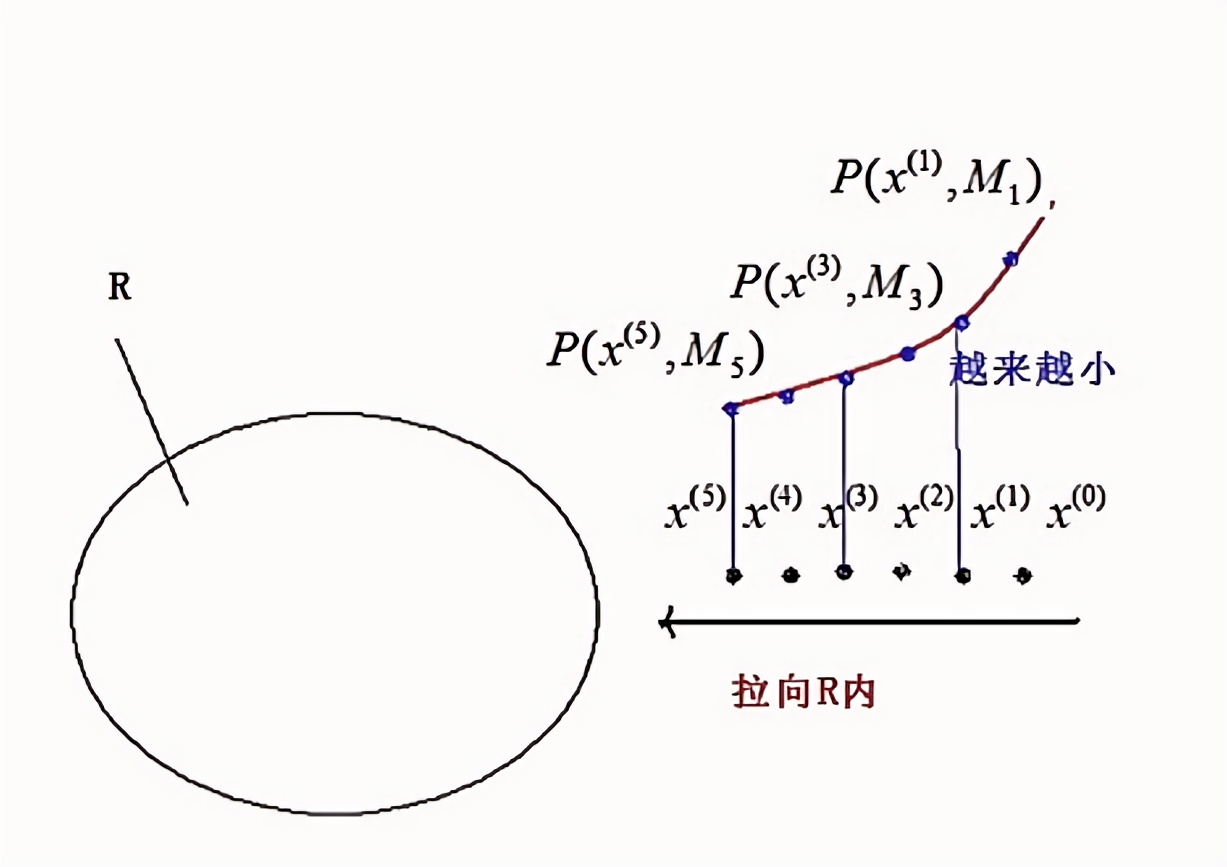
\includegraphics[width=0.5\textwidth]{./image/26.png}
    \caption{外点法示意图}
    \label{fig:Chapter4_Temporary_Pavilion_1}
\end{figure}


\subsubsection{内点法}
如果有把握将初始迭代点取在可行域R内,则可采用障碍函数法(内点法)来进行约束极值问题的无约束化\footnote{这一方法的主要思想是,找一个新的无约束目标函数,其中含有一个障碍项,障碍项的选取目的在于“在可行域的边界上设置一道障碍,使迭代点靠近边界时,新目标函数值迅速增长,从而阻止迭代点跑到可行域外面。”}。
\begin{notebox}{\textbf{障碍函数法}}{}
    \\类似于惩罚函数法,选择障碍项:
    \[
    \sum_{j=1}^{l} \frac{1}{g_j(x)} \quad \text{或} \quad \sum_{j=1}^{l} \log(g_j(x)),
    \]
    并以 \(\gamma_k\) 作为障碍因子(\(\gamma_k > 0\)),构造新的无约束目标函数:
    \[
    \min P(x, \gamma_k),
    \]
    其中
    \[
    P(x, \gamma_k) = f(x) + \gamma_k \sum_{j=1}^{l} \frac{1}{g_j(x)} \quad (\gamma_k > 0),
    \]
    或
    \[
    P(x, \gamma_k) = f(x) - \gamma_k \sum_{j=1}^{l} \log(g_j(x)) \quad (\gamma_k > 0).
    \]
    
    当 \(x\) 接近可行域边界时,\(g_j(x) \to 0\),从而 \(P(x, \gamma_k) \to \infty\)。
\end{notebox}
\textbf{说明}
    \begin{enumerate}
        \item 初始点必须选在可行域 \(R\) 内部,越靠近边界,障碍值越大。
        \item 所有迭代过程都在可行域 \(R\) 内进行,相当于求解无约束非线性规划问题。
    \end{enumerate}
\begin{figure}[H]
    \centering
    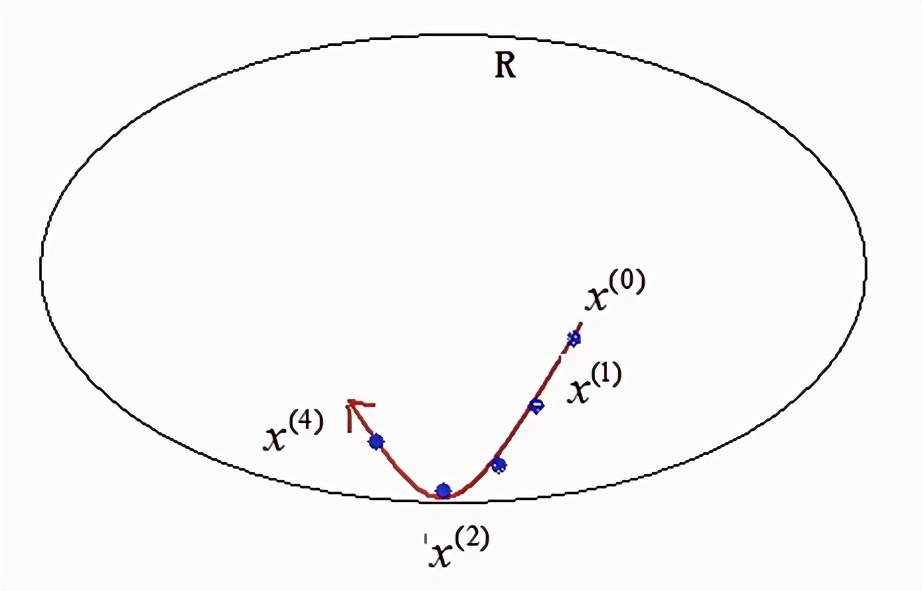
\includegraphics[width=0.5\textwidth]{./image/27.png}
    \caption{内点法示意图}
    \label{fig:Chapter4_Temporary_Pavilion_1}
\end{figure}

\subsection{逐次逼近类方法}
\label{sec:逐次逼近类方法}
这类方法\footnote{这类方法的主要思路是,通过对非线性函数加以台劳展开,并进行逐次逼近,将复杂的非线性函数简化为线性函数或简单非线性函数,再对此线性函数求线性规划,或对简单非线性函数求非线性规划(例如二次规划)。}主要由两种,逐次线性规划法和逐次二次规划法组成。
\subsubsection{逐次线性规划法(SLP)}
\begin{thmbox}{\textbf{线性规划的推出}}
针对如下问题:

\[
\min f(x), \quad g_j(x) \geq 0, \quad j = 1, 2, \dots, l
\]

设 \( x^{(k)} \) 是第 \( k \) 步选代点,则在 \( x^{(k)} \) 附近作泰勒展开:

\[
f(X) = f(X^{(k)}) + \nabla f^T(X^{(k)})(X - X^{(k)}) + o((X - X^{(k)})^2)
\]

\[
\approx f(X^{(k)}) + \nabla f^T(X^{(k)})(X - X^{(k)})
\]

\[
g_j(X) = g_j(X^{(k)}) + \nabla g_j^T(X^{(k)})(X - X^{(k)}) + o((X - X^{(k)})^2)
\]

\[
\approx g_j(X^{(k)}) + \nabla g_j^T(X^{(k)})(X - X^{(k)})
\]

代入原非线性规划中:

\[
\min f(X^{(k)}) + \nabla f^T(X^{(k)})(X - X^{(k)}), \quad g_j(X^{(k)}) + \nabla g_j^T(X^{(k)})(X - X^{(k)}) \geq 0, \quad j = 1, 2, \dots, l
\]

这就是关于 \( X \) 的线性规划。
\end{thmbox}

\textbf{说明:}
\begin{enumerate}
    \item 解上述线性规划,得到一个新的 \( X^{(k+1)} \),
    \begin{itemize}
        \item 若 \( X^{(k+1)} \in \) 可行域 \( R \),则可将 \( X^{(k+1)} \) 作为新点;
        \item 若 \( X^{(k+1)} \notin R \),则 \( X^{(k+1)} \) 为不可行点,此时应缩小步长,重新求取线性规划。
    \end{itemize}
    \item 在以上展开中,线性近似的前提条件是 \( X \) 距 \( X^{(k)} \) 足够近,所以为使得线性近似的误差不至太大,需要满足:
\[
\| X - X^{(k)} \| < \delta
\]
即下一个迭代点的步长应小于 \( \delta \)。
\end{enumerate}


\begin{notebox}{\textbf{算法流程}}{}
\begin{enumerate}
\item 设定初始点 \( X^{(0)} \) 和收敛精度因子 \( \epsilon > 0 \),令 \( k = 0 \)。
\item 计算目标函数的梯度 \( \nabla f(X^{(k)}) \) 和约束函数的梯度 \( \nabla g_j(X^{(k)}) \)。
\item 设定步长限制 \( \sigma^{(k)} \),解线性规划:

\[
\min f(X^{(k)}) + \nabla f^T(X^{(k)})(X - X^{(k)}), \quad g_j(X^{(k)}) + \nabla g_j^T(X^{(k)})(X - X^{(k)}) \geq 0, \quad j = 1, 2, \dots, l
\]

\[
\text{满足} \quad \| X - X^{(k)} \| < \sigma^{(k)}
\]
得到下一个迭代点 \( X^{(k+1)} \)。
\end{enumerate}
\end{notebox}
\subsubsection{逐次二次规划法(SQP)}
\begin{thmbox}{\textbf{二次规划的推出}}{}
    考虑优化问题:
    \[
    \min f(x), \quad \text{满足约束} \quad g_j(x) \geq 0, \quad j = 1, 2, \cdots, l'
    \]
    
    设 \( X^{(k)} \) 是第 \( k \) 步的迭代点,在 \( X^{(k)} \) 附近作泰勒展开:
    
    \begin{align*}
    f(X) &= f(X^{(k)}) + \nabla f^T(X^{(k)})(X - X^{(k)}) \\
    &\quad + \frac{1}{2}(X - X^{(k)})^T H(X^{(k)})(X - X^{(k)}) + o(\|X - X^{(k)}\|^2) \\
    &\approx f(X^{(k)}) + \nabla f^T(X^{(k)})(X - X^{(k)}) \\
    &\quad + \frac{1}{2}(X - X^{(k)})^T H(X^{(k)})(X - X^{(k)})
    \end{align*}
    
    式中,\( H(X^{(k)}) \) 是在 \( X^{(k)} \) 点的Hesse矩阵。
    
    \begin{align*}
    g_j(X) &= g_j(X^{(k)}) + \nabla g_j^T(X^{(k)})(X - X^{(k)}) + o(\|X - X^{(k)}\|) \\
    &\approx g_j(X^{(k)}) + \nabla g_j^T(X^{(k)})(X - X^{(k)})
    \end{align*}
    
    将近似表达式代入原非线性规划问题,得到:
    
    \begin{align*}
    &\min_X \left[ f(X^{(k)}) + \nabla f^T(X^{(k)})(X-X^{(k)}) + \frac{1}{2}(X-X^{(k)})^T H(X^{(k)})(X-X^{(k)}) \right] \\
    &\text{约束条件:} \quad g_j(X^{(k)}) + \nabla g_j^T(X^{(k)})(X-X^{(k)}) \geq 0, \quad j=1,2,\cdots,l'
    \end{align*}
    
\end{thmbox}
这是一个典型的二次规划(QP)问题。算法迭代流程与序列线性规划(SLP)中的流程结构相似。

\section{案例分析}
\begin{exbox}{发电机组的功率分配问题}{}
\textbf{例:}某发电厂现有三台发电机组并联运行,每台机组的发电功率可以在30~1600kW的范围内调节,
但功率越大,发电费用越高,试验表明,如果记三台机组的发电功率分别为$x_1,x_2,x_3$(单位:kW),
则相应的发电费用分别为$f_1(x_1)=2x_1^2+3x_1+1$,$f_2(x_2)=x_2^2+4x_2+2$,$f_3(x_3)=x_3^2+x_3+6$
,现要求三台发电机组的总功率为3500kW,试问各发电机组应如何分配负荷(功率)使得总
发电费用最低?
\\
\textbf{解:}设三台机组的发电功率$x_1,x_2,x_3$为决策变量,以三台机组的发电总费
用为目标函数,考虑到所需要的总功率和各机组的功率范围作为约束,建立如下的优化模型:
$$
\min f=f(x_1)+f(x_2)+f(x_3)
$$
$$
s.t.
\begin{cases}
    x_1+x_2+x_3=3500 \\
    30 \leq x_1,x_2,x_3 \leq 1600 \\
\end{cases}
$$
\end{exbox}
\ifx\allfiles\undefined
	% 如果有这一部分的参考文献的话,在这里加上
	% 没有的话不需要
	% 因此各个部分的参考文献可以分开放置
	% 也可以统一放在主文件末尾。
	
	%  bibfile.bib是放置参考文献的文件,可以用zotero导出。
	% \bibliography{bibfile}
	
	end{document}
	\else
	\fi